\documentclass{beamer}
\usetheme{CENIDETDIE}
\setbeamertemplate{caption}[numbered]
\usefonttheme[onlymath]{serif}

% ------------------------------------------------------------------------------------------------

\usepackage[utf8]{inputenc}
\usepackage[T1]{fontenc}
\usepackage{helvet}
\usepackage{graphicx} % Allows including images
\usepackage{booktabs} % Allows the use of \toprule, \midrule and \bottomrule in tables
\numberwithin{figure}{section}
\numberwithin{equation}{section}
\usepackage[square,sort,comma,numbers]{natbib}
\usepackage{ragged2e}
\usepackage{caption}
\usepackage{subcaption}
\usepackage{mathabx}

 

% ------------------------------------------------------------------------------------------------

\title{WORK PROGRESS}
%\subtitle{Presentation in Beamer-\LaTeX}
\author{Saeed ZAHRAN $^{1}$ }
\institute{$^{1}$UNIVERSITÉ DE PICARDIE JULES VERNE \\ 
		}
\date{\today}

\begin{document}

% ------------------------------------------------------------------------------------------------

\begin{frame}[plain,t]
\titlepage
\end{frame}

% ------------------------------------------------------------------------------------------------

\begin{frame}[plain,noframenumbering]
  \addtocounter{framenumber}{-1}
  \scriptsize
%   \thispagestyle{empty}
  \frametitle{Indice}
  \setbeamertemplate{section in toc}[sections numbered]
  \tableofcontents[hideallsubsections]
\end{frame}

% ------------------------------------------------------------------------------------------------

\section{RDF previous }
\begin{frame}
 \frametitle{RDF previous }
 \scriptsize
 \justifying
  RDF was original writeen by Tim Bray in 1998 an update by Dan Brickley in 2001\cite{w3:2004:w3c}.\\ 
  \vspace{5mm}
  The Resource Description Framework (RDF) is a lenguage for representing information about resources in the World Wide Web\cite{w3:2004:w3c}.\\
  \vspace{5mm}
 RDF descriptions, often contain redundancies, and could be generated differently even when describing the same resources, which would have a negative impact on various RDF-based applications (e.g.,RDF storage, processing time, loading time, similarity measuring, mapping, alignment, and versioning)\cite{TiconaUltimo}.

\end{frame}

% ------------------------------------------------------------------------------------------------

\section{RDF definition}
\begin{frame}
 \frametitle{RDF definition}
 	\textbf{RDF graph:} set of triples 
 	\begin{figure}
        \centering
        \begin{subfigure}[h]{0.45\textwidth} 
            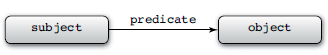
\includegraphics[width=\textwidth]{pictures/rdf_begin}
            \label{fig:rdf_begin}
        \end{subfigure}       
        \begin{subfigure}[h]{0.45\textwidth} 
            
\includegraphics[width=\textwidth]{pictures/RDF_begin2}
            \label{fig:rdf_begin2}
        \end{subfigure}
        \caption{Example of RDF triple}
    \end{figure}

 	\justify There can be three kinds of nodes: IRIs, literals, and blank nodes.
	\begin{itemize}
    \footnotesize
    \vspace{5mm}
    \item  \justify \textbf{IRI} (Internationalized Resource Identifier) refers to a resource (the referent).
    \item  \justify \textbf{Literal} denotes resources which have an associated value for example, an integer or string value.
    \item  \justify \textbf{Blank nodes} are local identifiers which do not identify specific resources.
	\end{itemize}

\end{frame}

% ---------------------------------------------------------------------------------------
\section{}
\begin{frame}
 \frametitle{RDF definition}
 	RDF data graph and RDF schema graph:
 	
 	\begin{figure}[p]
  		\centering
  		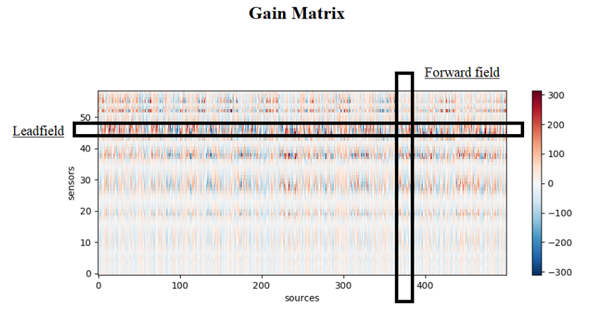
\includegraphics[width=1.0\linewidth]{pictures/lf}
  		\caption{\scriptsize Advantages of RDF summarization}
  		\label{fig:approaches_RDF}
 	\end{figure}
    
\end{frame}

% ------------------------------------------------------------------------------------------------







%----------------------------------------------
\section{}
\begin{frame}
 \frametitle{RDF definition}
  

 	\begin{figure}[h]
        \begin{subfigure}[h]{0.53\linewidth} 
            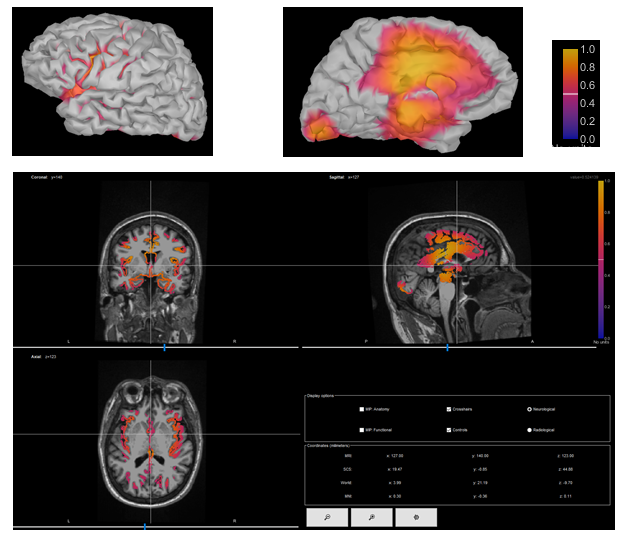
\includegraphics[width=\linewidth]{pictures/meg1}
            \caption{\tiny RDF graph}
            \label{fig:rdf_graph}
        \end{subfigure}       
        \begin{subfigure}[h]{0.45\linewidth} 
            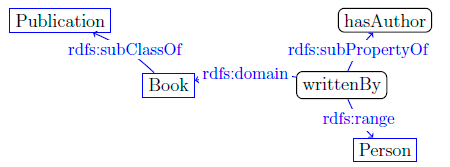
\includegraphics[width=\linewidth]{pictures/rdfs_graph}
            \caption{\tiny RDF Shema (RDFS) graph}
            \label{fig:rdfs_graph}
        \end{subfigure}
       % \caption{\scriptsize Example of RDF graph and RDFS graph}
    \end{figure}

  
\end{frame}

% ------------------------------------------------------------------------------------------------
\section{}
\begin{frame}
 \frametitle{Two}
  

 	\begin{figure}[h]
        \begin{subfigure}[h]{0.53\linewidth} 
            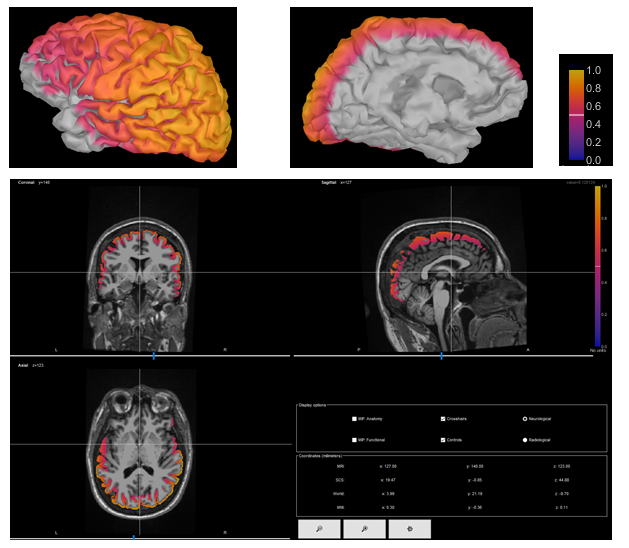
\includegraphics[width=\linewidth]{pictures/meg2}
            \caption{\tiny RDF graph}
            \label{fig:rdf_graph}
        \end{subfigure}       
        \begin{subfigure}[h]{0.45\linewidth} 
            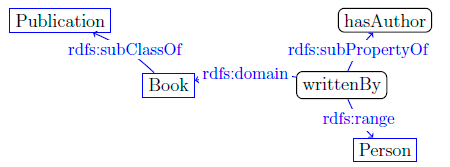
\includegraphics[width=\linewidth]{pictures/rdfs_graph}
            \caption{\tiny RDF Shema (RDFS) graph}
            \label{fig:rdfs_graph}
        \end{subfigure}
       % \caption{\scriptsize Example of RDF graph and RDFS graph}
    \end{figure}

  
\end{frame}



%------------------------------
\section{}
\begin{frame}
 \frametitle{Three}
  

 	\begin{figure}[h]
        \begin{subfigure}[h]{0.53\linewidth} 
            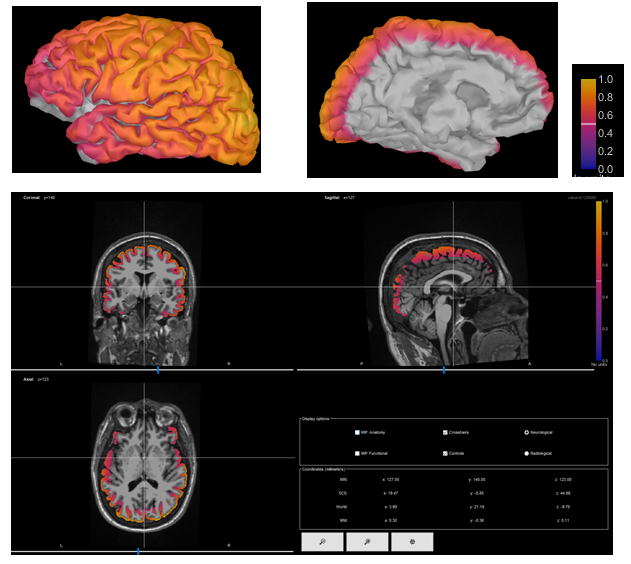
\includegraphics[width=\linewidth]{pictures/meg3}
            \caption{\tiny RDF graph}
            \label{fig:rdf_graph}
        \end{subfigure}       
        \begin{subfigure}[h]{0.45\linewidth} 
            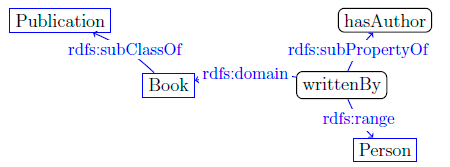
\includegraphics[width=\linewidth]{pictures/rdfs_graph}
            \caption{\tiny RDF Shema (RDFS) graph}
            \label{fig:rdfs_graph}
        \end{subfigure}
       % \caption{\scriptsize Example of RDF graph and RDFS graph}
    \end{figure}

  
\end{frame}




%-----------------
\section{Advantages of RDF}
\begin{frame}
 \frametitle{Advantages of RDF}
 \begin{itemize}
	\scriptsize
  	\item Efforts to generate knowledge base of RDF scalable, fast, secure\cite{Ren2018}.
    \vspace{2.5mm}
  	\item Efforts to incorporate data quality metrics in RDF queries \cite{Zneika2016}\cite{Cheng2012}\cite{Bursztyn2014}.
    \vspace{2.5mm}
  	\item  Efforts to process multiple RDF networks in parallel \cite{Doel2017}\cite{Kushwaha2015}.
    \vspace{2.5mm}
    \item  Efforts to consult information in RDF based on data patterns, keywords\cite{Kushwaha2015}.
 \end{itemize}
 
\end{frame}

% ------------------------------------------------------------------------------------------------

\section{Problems in RDF representation}
\begin{frame}
 \frametitle{Problems in RDF representation}
 \begin{enumerate}
	\scriptsize
  	\item RDF datasets are growing constantly.
    \vspace{2.5mm}
  	\item Minimum Constraints for RDF data make it irregular, difficult to comprehend and visualize, this can cause problems for information extraction, processing, and analysis.\label{item:2}
    \vspace{2.5mm}
  	\item  RDFs have been designed as a query standard based on explicit and implicit data.\label{item:3}
 \end{enumerate}
 \vspace{5mm}
 \centering
 Many authors propose use \textbf{RDF summarization} approach to solve problem  item~\ref{item:2} y ~\ref{item:3}
 
 
\end{frame}

% ------------------------------------------------------------------------------------------------

\section{RDF summarization}
\begin{frame}
 \frametitle{RDF summarization}
 \justify \scriptsize

 RDF graph are often large and varied, produced in a variety of contexts such as social networks, medical data, scientific data, etc. \cite{Manolescu2018a}. The large amount of data contained in the RDF is often too expensive to perform queries to acquire information.
\vspace{3mm}
The RDF summary refers to the process of extracting concise but significant summaries of RDF Knowledge Bases (KBs) that represent as close as possible the actual contents of the KB, both in terms of structure and data \cite{Zneika2018}.

 \end{frame}
 
% ------------------------------------------------------------------------------------------------

\subsection{RDF summary requerimients}
\begin{frame} 
 \frametitle{RDF summary requerimients}
 \normalsize We are interested in extracting a summary graph, having the following characteristics:
 \vspace{5mm}
  \begin{itemize} \scriptsize
  	\item \justify The summary is a RDF graph: The summary graph should be a RDF graph itself.
    \vspace{2mm}
  	\item \justify The size of the Summary: The volume of a graph is the numbers of its edges and nodes.   
    		\\Thus the summary graph should:
    \vspace{2mm}
  		\begin{itemize}	\scriptsize
    		\item \justify Be smaller than the original RDF graph.
    		\vspace{2mm}
    		\item Contain all the important information.
            \vspace{2mm}
  			\item Report the most representative nodes (classes) and edges (properties).
 		\end{itemize}
  \end{itemize}

\centering 
\vspace{5 mm}\normalsize
\textbf{Interest in research towards the quality of the summary\cite{Khatchadourian2010}\cite{Zneika2018}}
 
\end{frame}
% ------------------------------------------------------------------------------------------------
\subsection{Main Approaches for RDF Summarization }
\begin{frame} \scriptsize
 \frametitle{Main Approaches for RDF Summarization\cite{Zneika2018}}
	\begin{figure}[p]
  		\centering
  		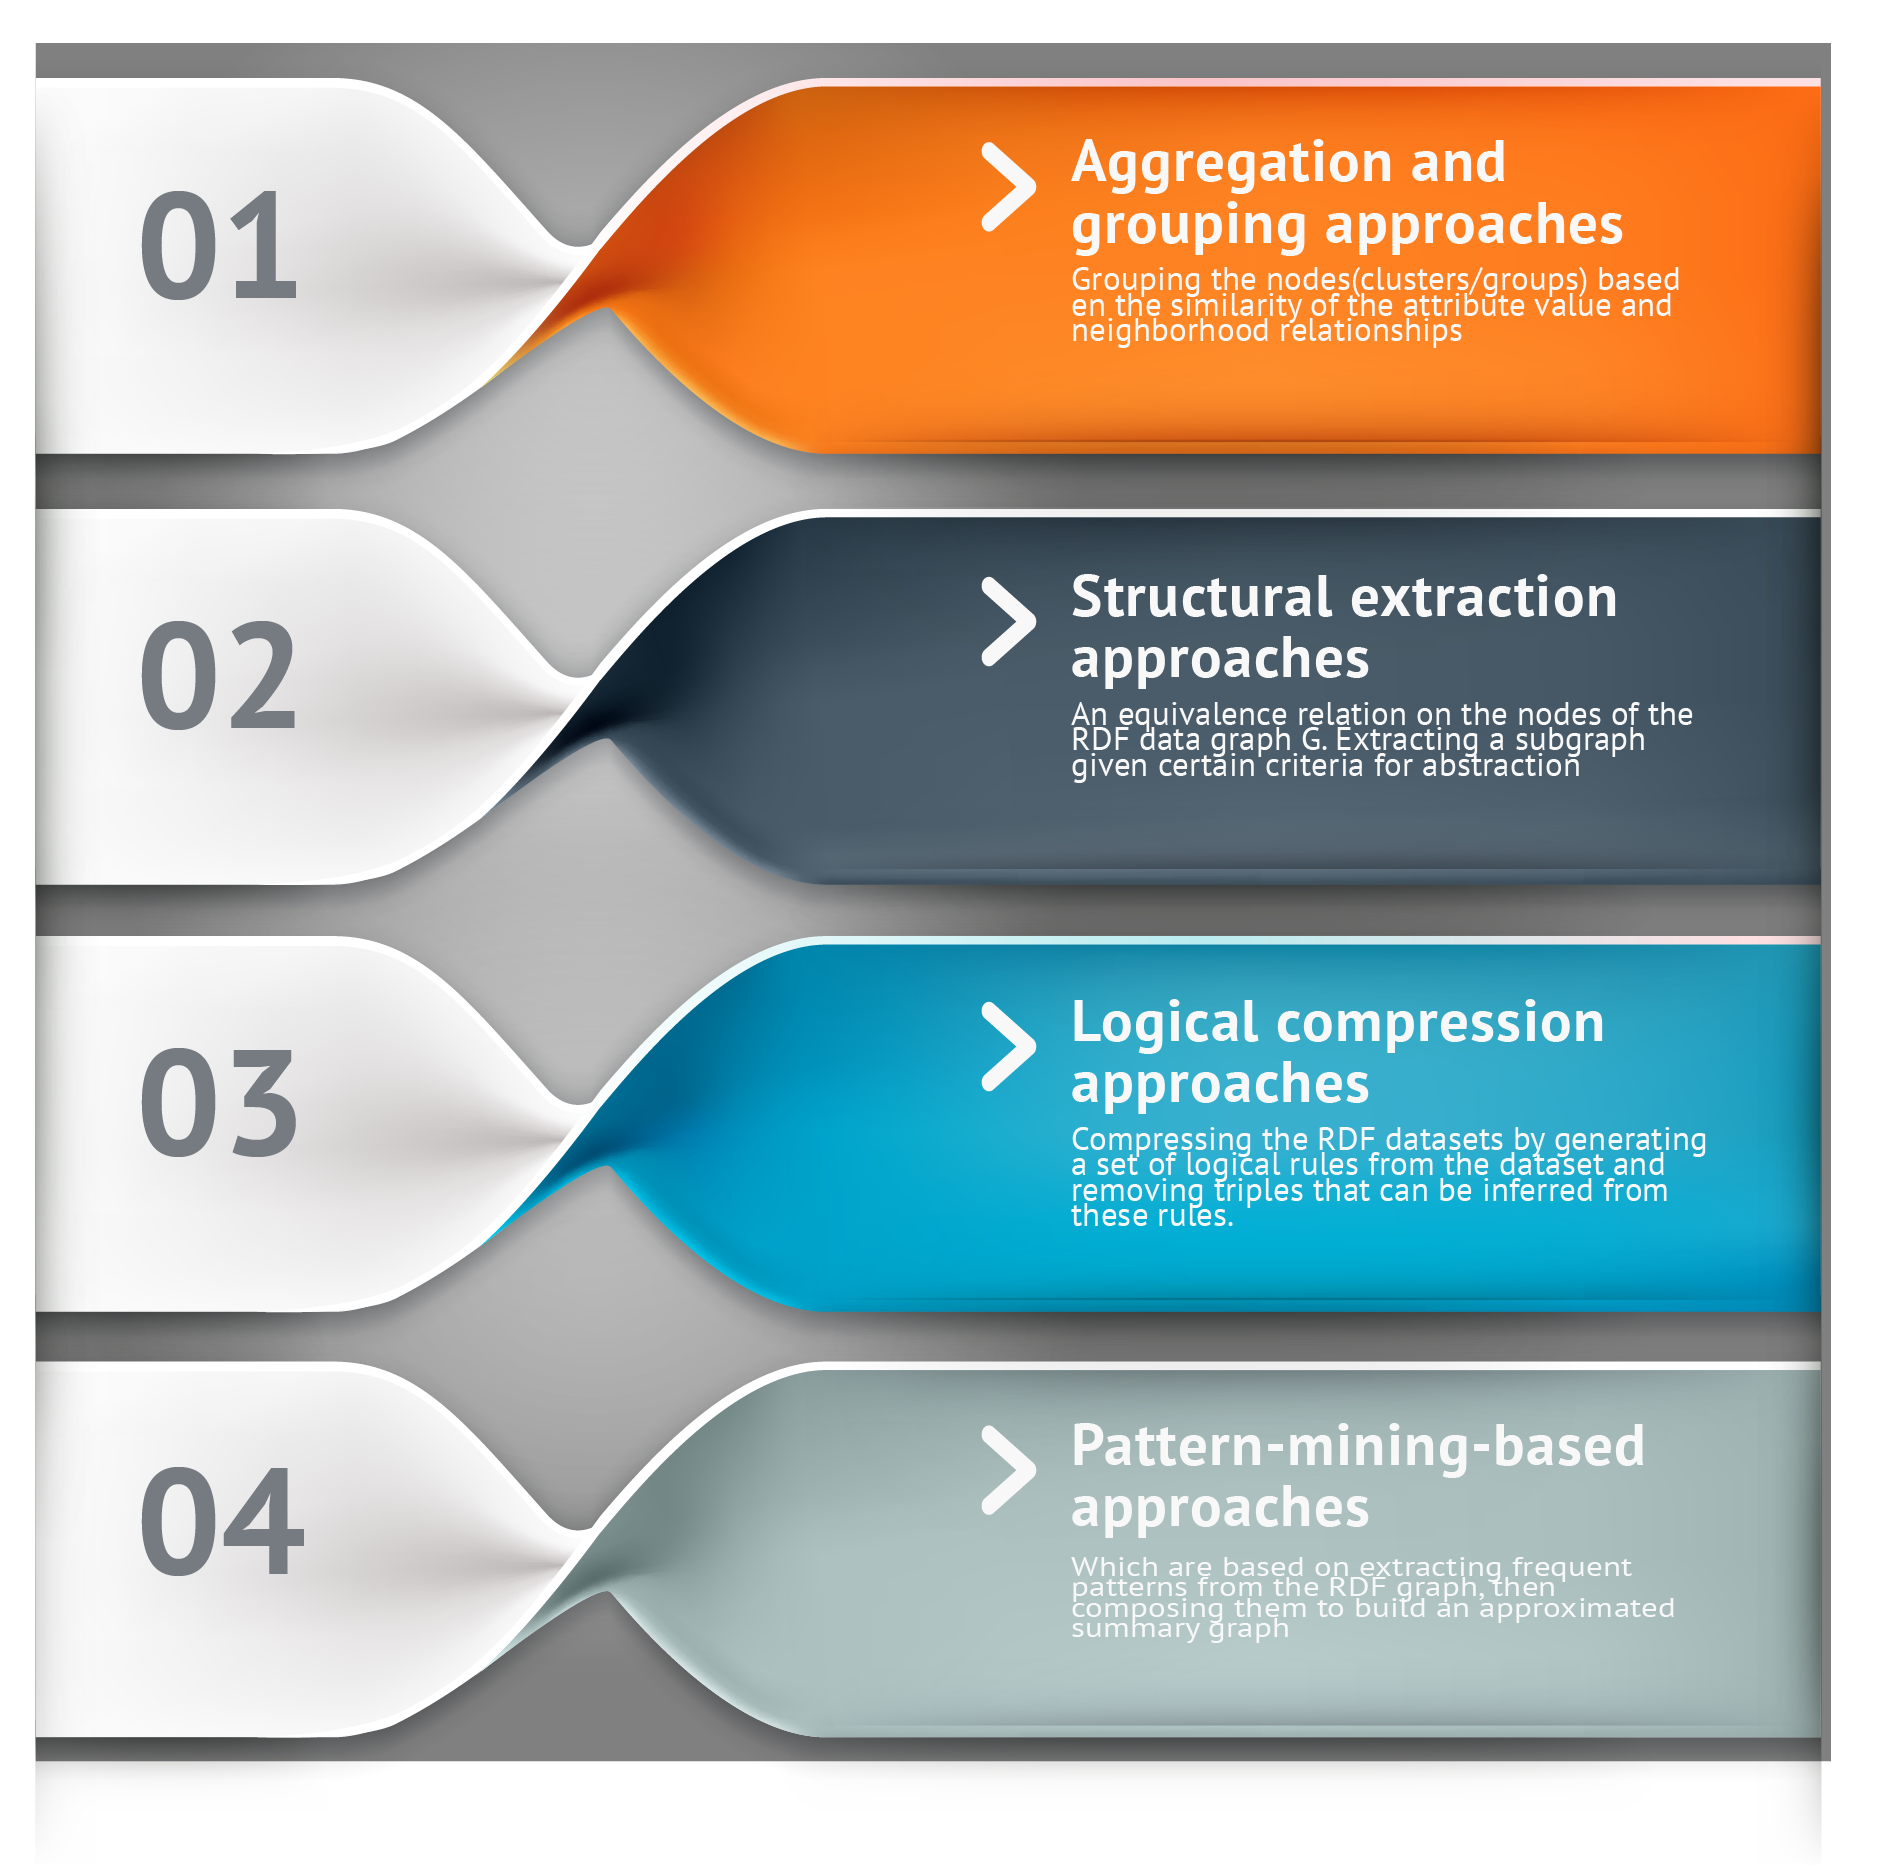
\includegraphics[width=0.7\linewidth]{pictures/approaches_RDF}
  		\caption{\scriptsize Main Approaches for RDF Summarization\cite{Zneika2018}}
  		\label{fig:approaches_RDF}
 	\end{figure}
 
 
\end{frame}
% ------------------------------------------------------------------------------------------------

\section{Advantages of RDF summarization}
\begin{frame} \scriptsize
 \frametitle{Advantages of RDF summarization}
  \begin{columns}[c] 
 	\column{.45\textwidth} % Left column and width
 		\begin{itemize} \justifying
        	
  			\item Efforts to manage heterogeneous and homogeneous RDF networks\cite{Aufaure2012}.
      		\vspace{2mm}
  			\item Efforts to obtain quality summaries\cite{Khatchadourian2010}.
      		\vspace{2mm}
    		\item Efforts to reduce the loss of information in RDF summaries.
      		\vspace{2mm}
    		\item Efforts to interpret explicit and implicit information in RDF summaries\cite{Ristoski}.
  		\end{itemize}

 	\column{.5\textwidth} 
 		\begin{figure}[p]
  		\centering
  		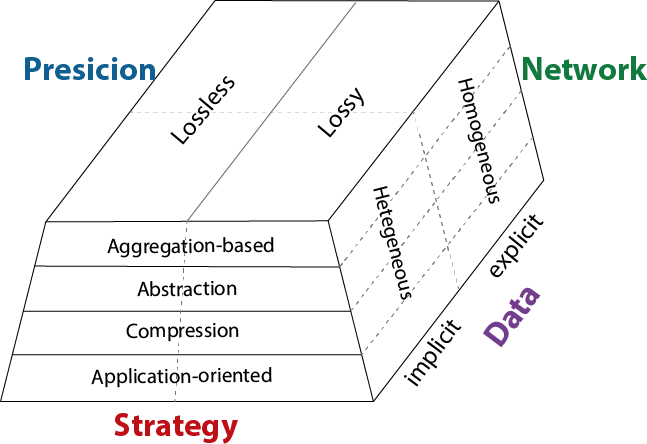
\includegraphics[width=1.0\linewidth]{pictures/strategyRDF}
  		\caption{\scriptsize Advantages of RDF summarization}
  		\label{fig:approaches_RDF}
 	\end{figure}
        
        
 \end{columns}
 

\end{frame}
% ------------------------------------------------------------------------------------------------


\section{Our Proposal: RDF graph summarization with RNN}
\begin{frame} \scriptsize  \justifying
 \frametitle{Our Proposal: RDF graph summarization with Recurrent Neural Network (RNN)}

In the paper: \textbf{“Modeling Relational Data with Graph Convolutional Networks”}\cite{Schlichtkrull2017}, exist some impressions:
\begin{itemize} \justifying
        	
  			\item General Fourier transform scales poorly with size of data so we need relaxations, normally use for image processing, where actual spatial convolutions are easy to compute.
      		\vspace{2mm}
  			\item At all levels in this network, the filters are limited to 3x3 in size and are also essentially fixed to be the same kernel across all layers and all units in entire network 
            \end{itemize}

\vspace{3mm}
In the paper  \textbf{“Convolutional Neural Networks on Graphs with Fast Localized Spectral Filtering”}\citet{Bresson2016}, the authors try to solve the above problems including higher order Chebyshev polynomials in the approximation.

\vspace{3mm}
\begin{alertblock}{}\normalsize
\justify \setlength{\parskip}{-5mm}
  For satisfy the stationarity, locality, compositionality 	 assumptions, we propose use \textbf{"Recurrent Neural Networks"}
 \end{alertblock}
\end{frame}
% ------------------------------------------------------------------------------------------------

\subsection{RDF summarization with RNN}
\begin{frame}
 \frametitle{RDF summarization with Recurrent Neural Network (RNN)}
 
 	\begin{figure}[p]
  		\centering
  		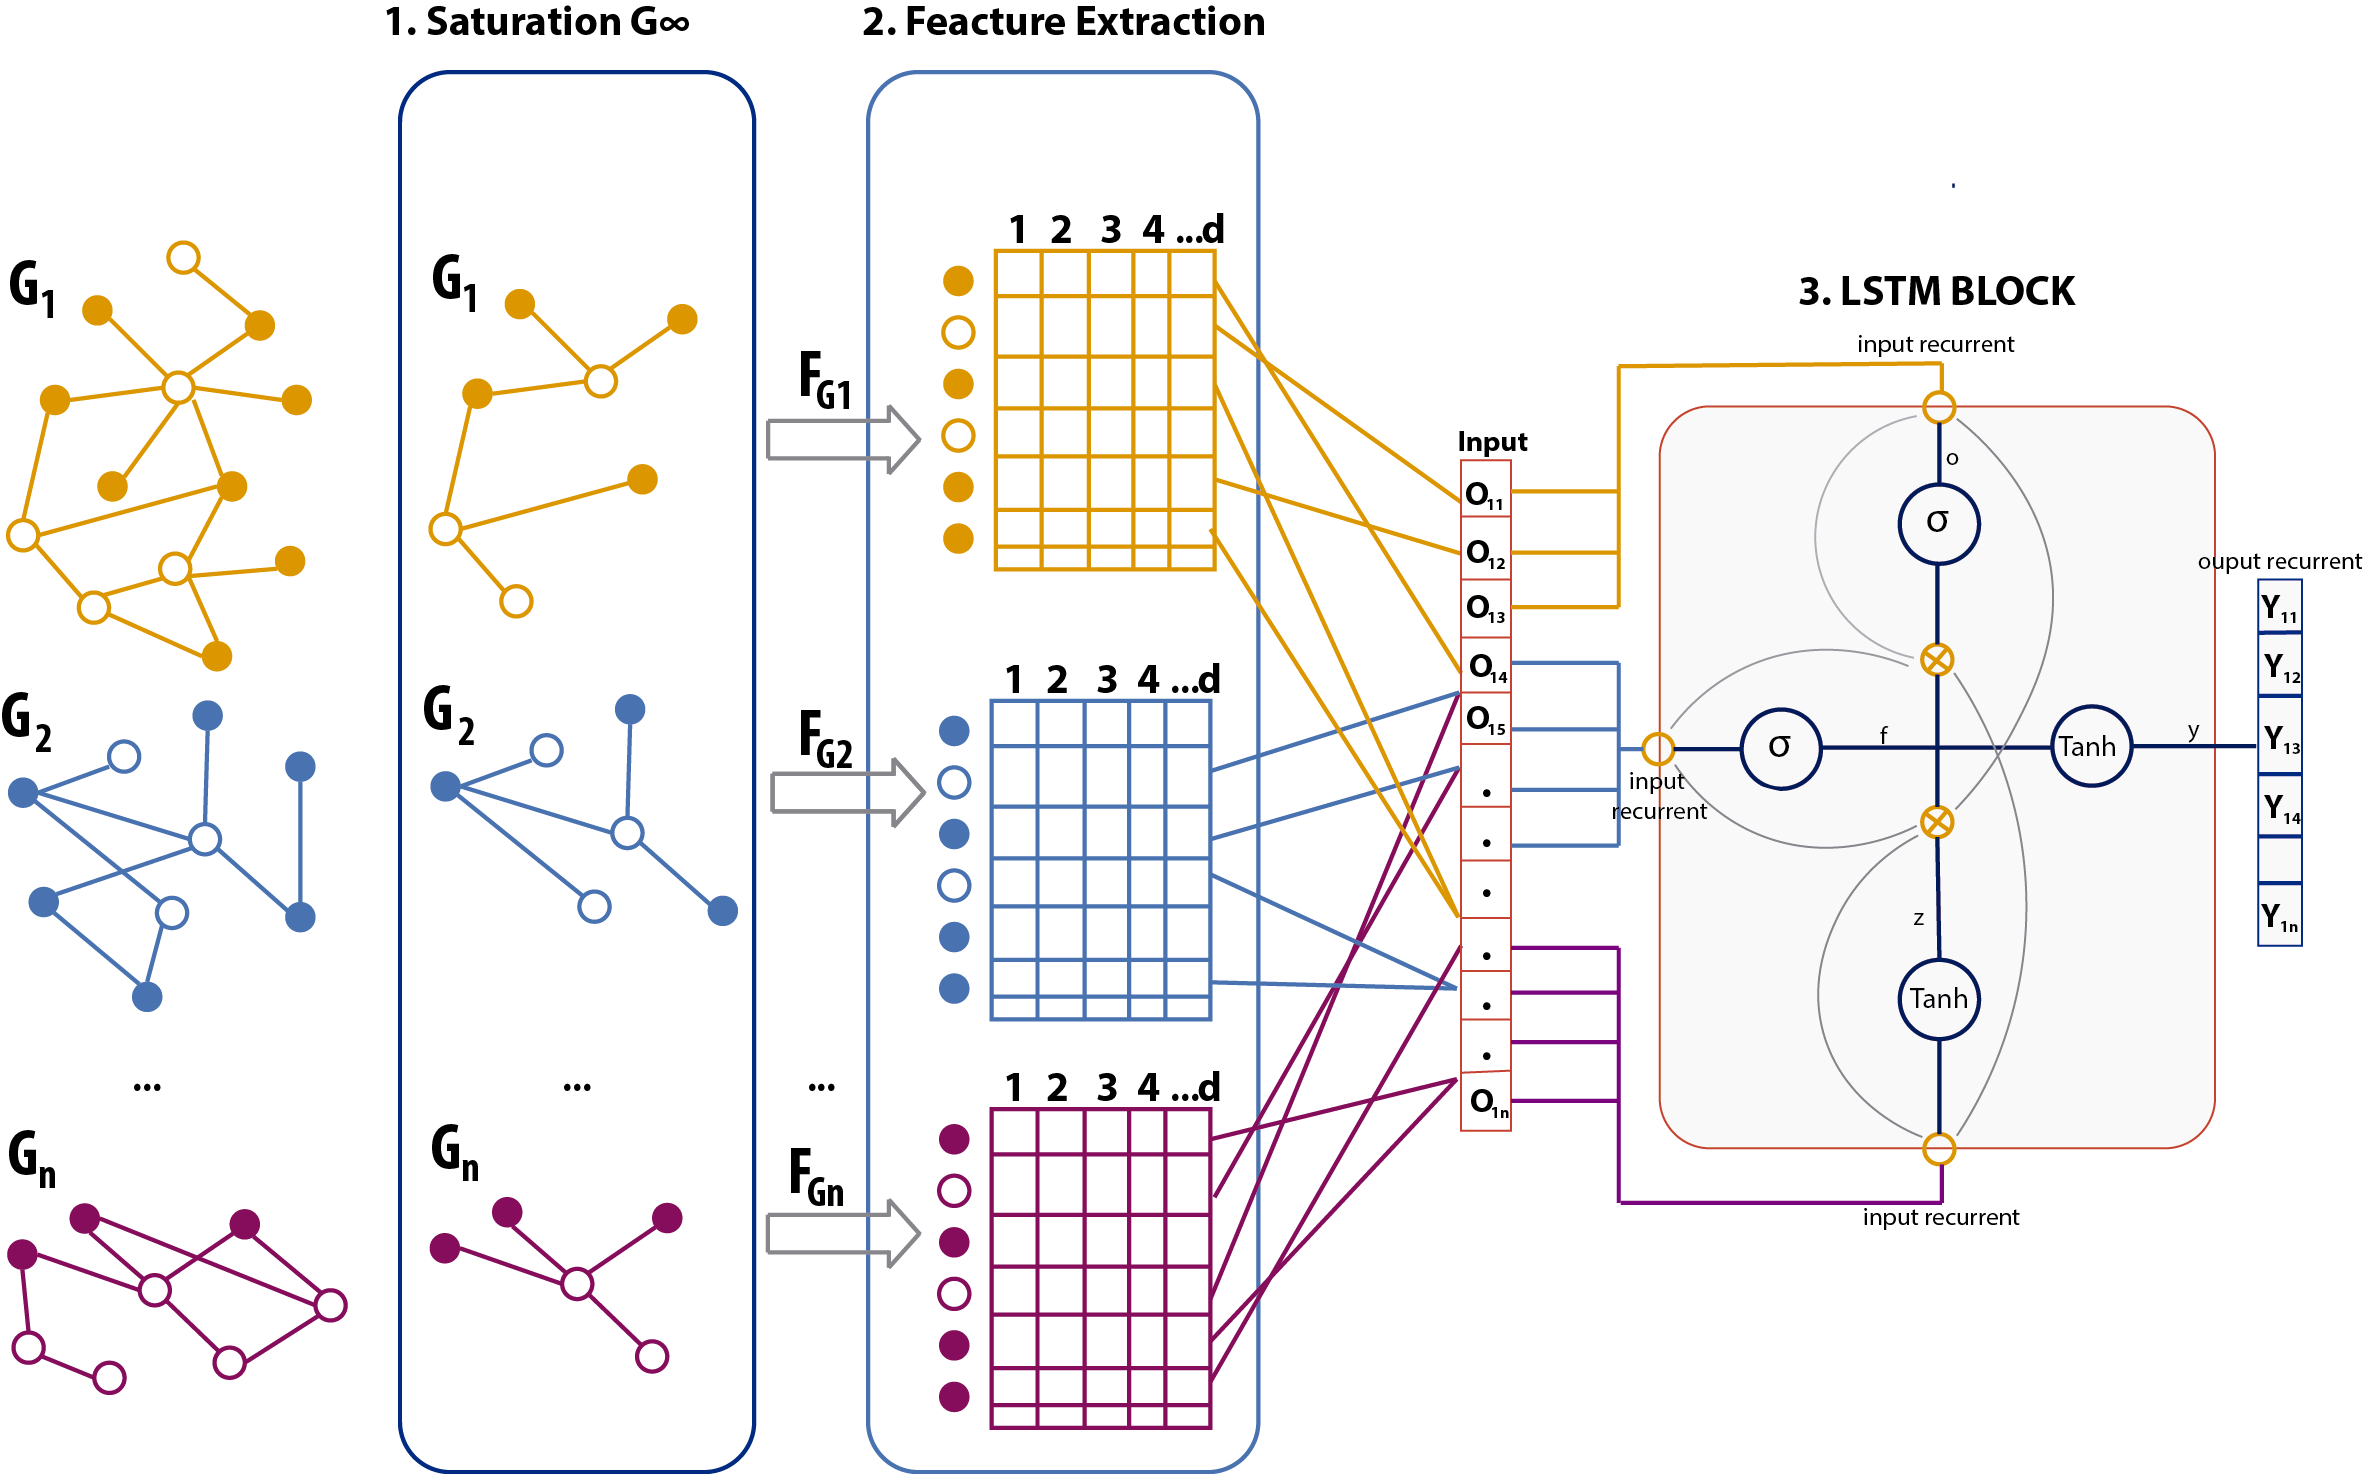
\includegraphics[width=1.0\linewidth]{pictures/ModeloRDF_RNN}
  		\caption{\scriptsize RDF graph summarization with RNN}
  		\label{fig:RDFRNN}
 	\end{figure}
 
\end{frame}
% ------------------------------------------------------------------------------------------------

\subsubsection{Saturation }
\begin{frame} \scriptsize \justifying
 \frametitle{Saturation}
 \begin{columns}[c] 
 	\column{.6\textwidth} % Left column and width
 		\begin{figure}[p]
  		\centering
  		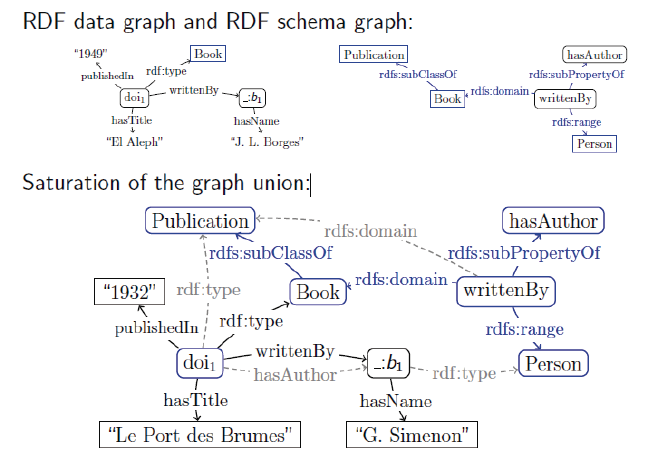
\includegraphics[width=1.0\linewidth]{pictures/RDF_RDFS_Saturacion}
  		\caption{\tiny Saturation of the graph union}
  		\label{fig:approaches_RDF}
 	\end{figure}
 	\column{.40\textwidth} 
 		\begin{figure}[p]
  		\centering
  		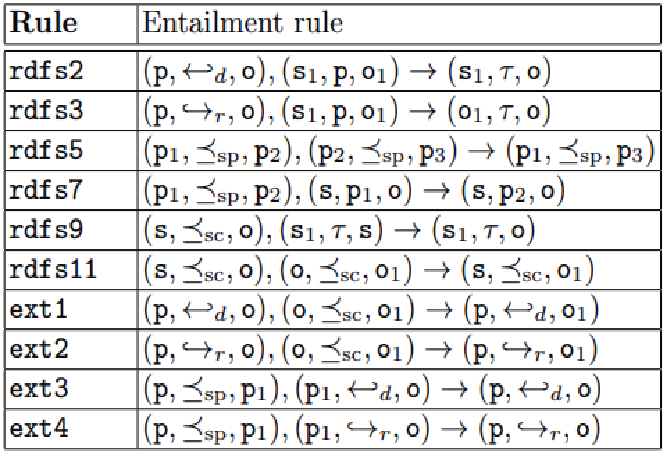
\includegraphics[width=1.0\linewidth]{pictures/Rule_RDFS}
  		\caption{\tiny Sample RDF entailment rules\cite{Hassad2017a}}
  		\label{fig:approaches_RDF}
 	\end{figure}
 \end{columns}
 
 
 \definecolor{rojo}{RGB}{255,39,8} 
 \vspace{3mm}
 \textcolor{rojo}{Other authors}\cite{Trisedya2018}\cite{Schlichtkrull2017}  assign labels to entity types, for example: “John Doe”, “London”, “England”, and “1967-01-10” can be mapped to “PERSON”, “CITY”, “COUNTRY”, and “DATE” 
 
\end{frame}
% ------------------------------------------------------------------------------------------------

\subsubsection{Feature extraction  }
\begin{frame} \scriptsize \justifying
 \frametitle{Feature extraction}
   \begin{columns}[c] 
 	\column{.45\textwidth} % Left column and width
 	\begin{figure}[p]
  		\centering
  		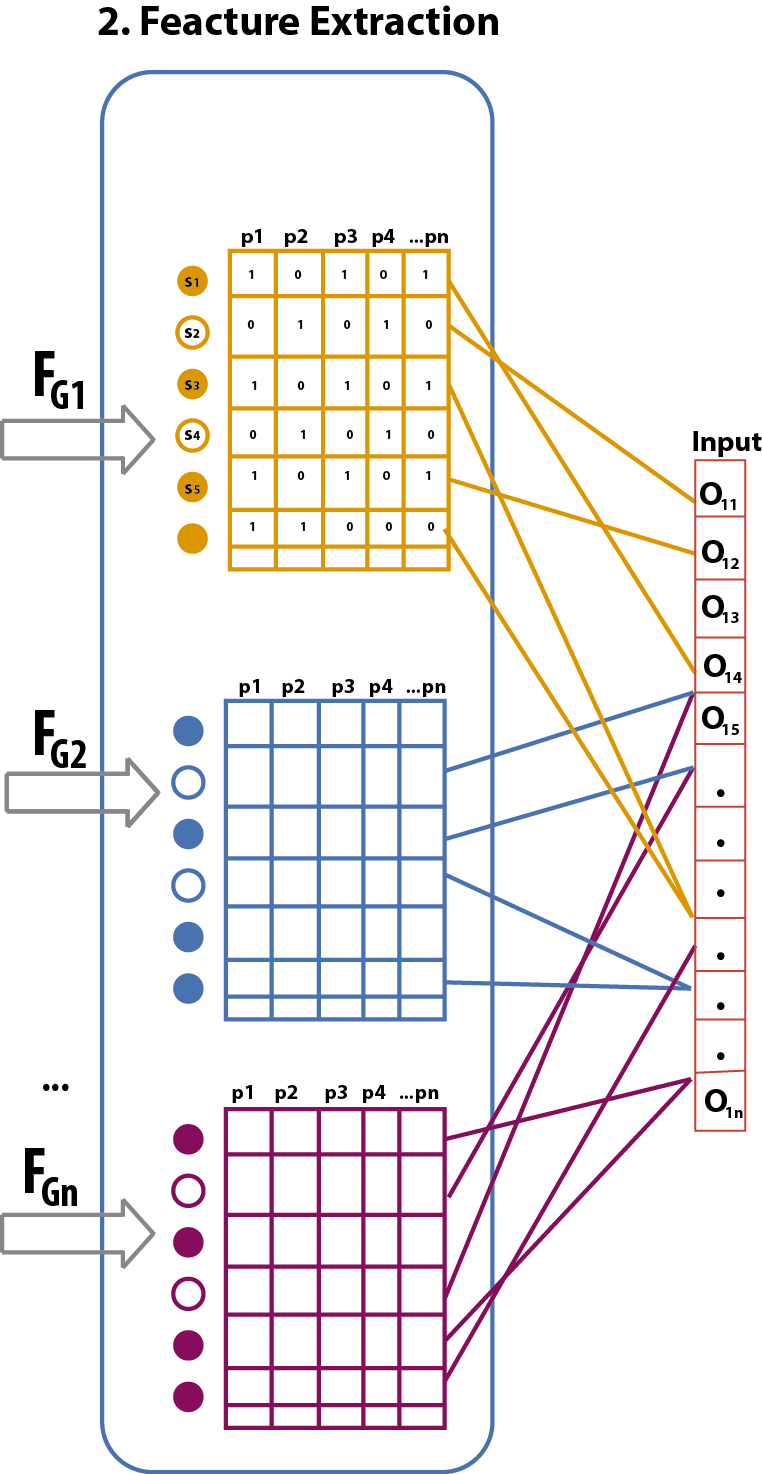
\includegraphics[width=0.7\textwidth]{pictures/feacture_extraction}
  		\caption{\tiny Feacture Extraction}
  		\label{fig:feacture_extraction}
 	\end{figure}
 	\column{.5\textwidth} 
    Other technique for feacture extraction\cite{Aufaure2012}
    \begin{figure}[p]
  		\centering
  		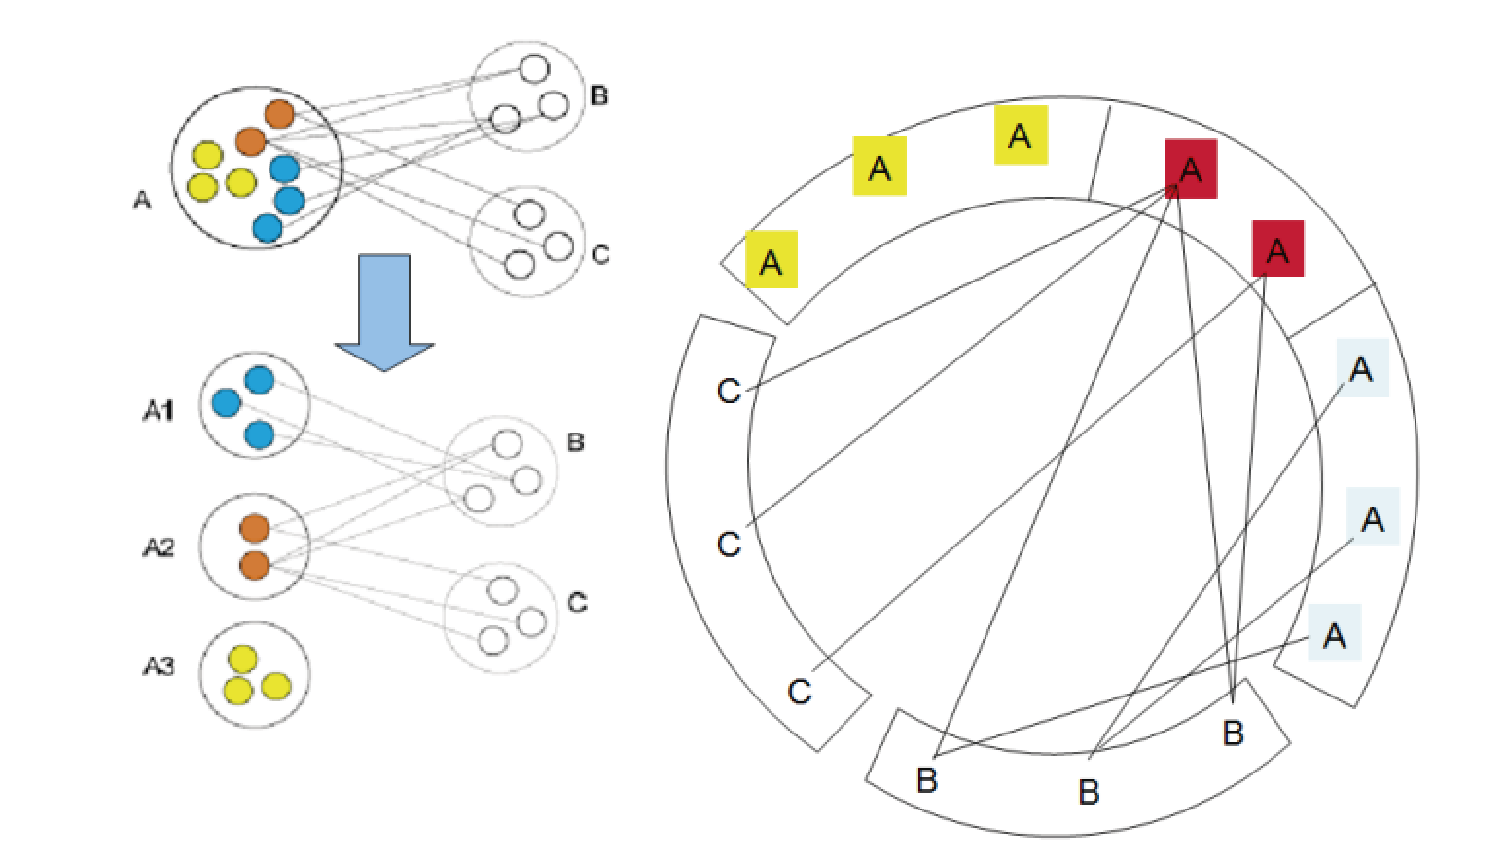
\includegraphics[width=1.0\linewidth]{pictures/ksnap}
  		\caption{\tiny Example of aggregation using K-Snap}
  		\label{fig:ksnap}
 	\end{figure}
  
 \end{columns}
 
 
 
 
\end{frame}
% ------------------------------------------------------------------------------------------------

\subsubsection{Recurrent Neural Networks}
\begin{frame}\justifying \scriptsize
 \frametitle{Recurrent Neural Networks}
 	\begin{figure}[p]
  		\centering
  		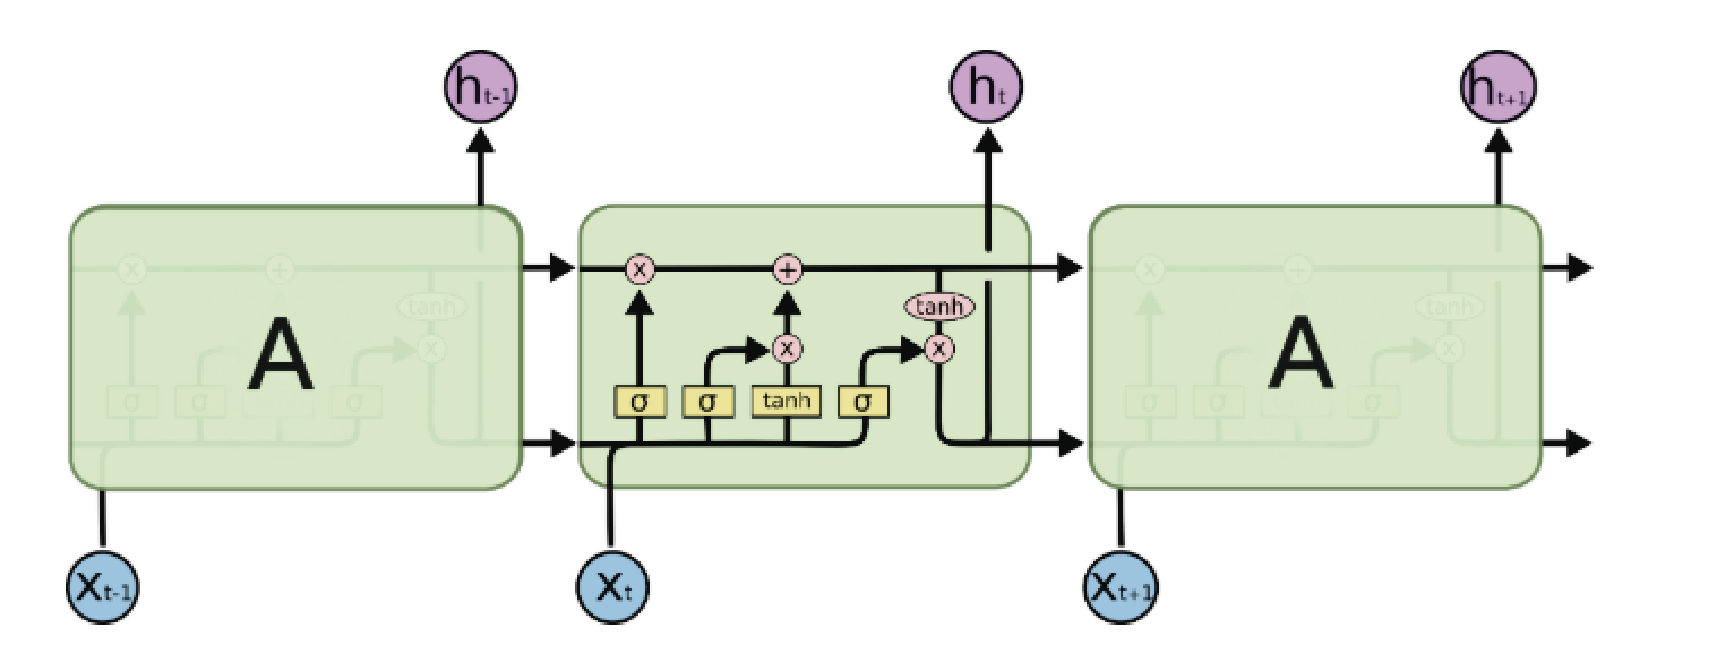
\includegraphics[width=0.7\textwidth]{pictures/RNN}
  		\caption{\tiny Recurrent Neural Networks Architecture}
  		\label{fig:feacture_extraction}
 	\end{figure}
    \begin{figure}[p]
  		\centering
  		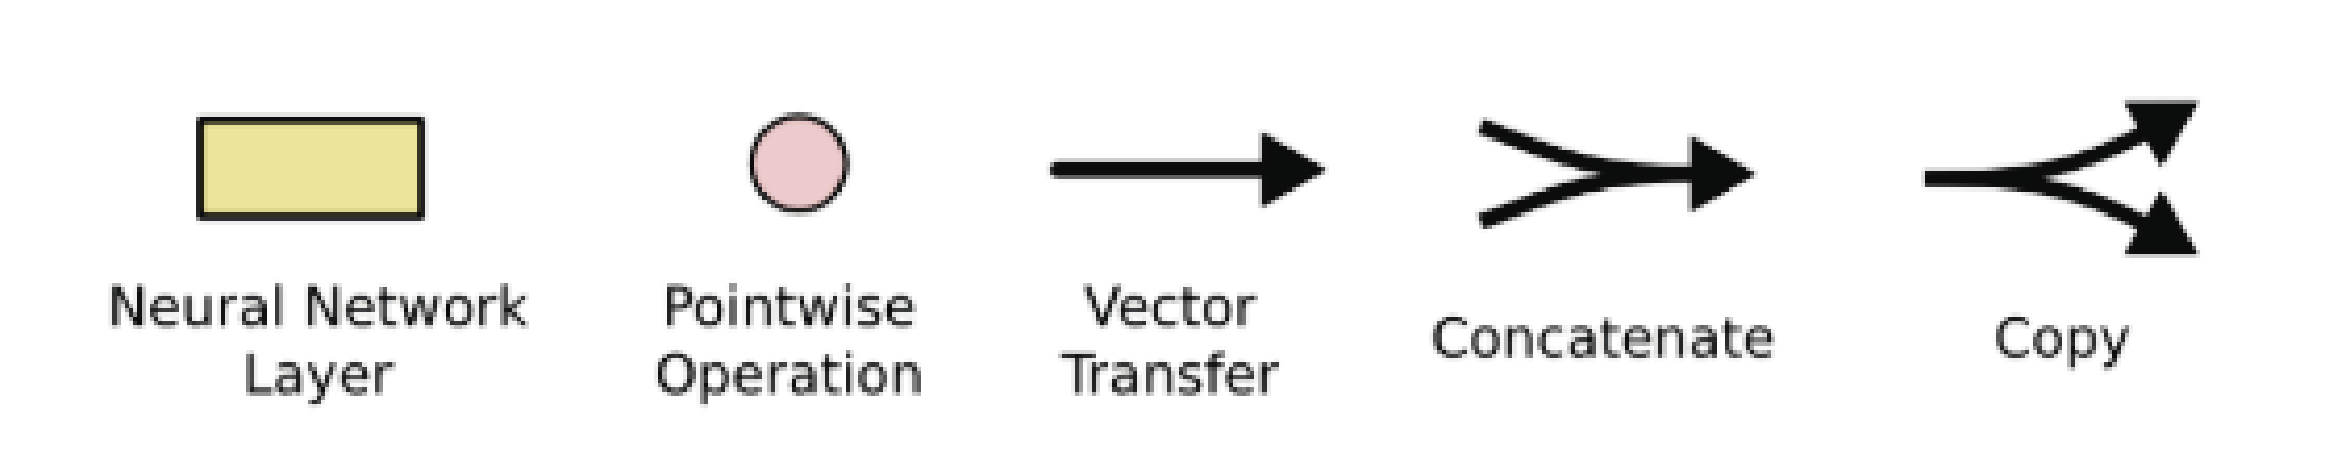
\includegraphics[width=0.6\textwidth]{pictures/leyendarnn}
  		\caption{\tiny Recurrent Neural Networks Architecture}
  		\label{fig:feacture_extraction}
 	\end{figure}
    
    \scriptsize Recurrent neural networks address the problem reasoning about previous events in the nodes to inform later ones. They are networks with loops in them, allowing information to persist\cite{Jozefowicz2015}.
\end{frame}

% ------------------------------------------------------------------------------------------------

\begin{frame}[allowframebreaks]{References} \justify \tiny
 \setbeamertemplate{bibliography item}[text]
 \bibliographystyle{apalike}
 \bibliography{references.bib}{}
\end{frame}

% ------------------------------------------------------------------------------------------------

\ThankYouFrame

% ------------------------------------------------------------------------------------------------

\end{document}
